\chapter{Bayesian periodization of postembryonic CMZ activity}
\label{chap:CMZ}
\section{Synopsis}
This study was organized to determine how postembryonic CMZ RPCs differ, if at all, from their embryonic counterparts. Because of the decreasing optical accessibility of the retina, and difficulties associated with marking cohorts of cells in live fish, we used CMZ RPC data from cryosections, which were related to the whole retina in a series of simulations. 

\section{Preliminaries: Calculation of Bayesian evidence supports independent Log-Normal modelling of CMZ parameters}
To take up the question of how CMZ RPC activity evolves over time, we measured CMZ and retinal parameters in histological studies of cryosections of zebrafish eyes harvested over the first year of the animal's life. We wish to extract as much information as possible about the structure and time-evolution of the CMZ population as a whole, in order to know how to best model its constituent RPCs. The initial approach is to geometrically impute measurements whole-eye CMZ and retinal volume from sample central cryosections, calculated as described in \autoref{sec:lenspopest}. These derived measurements form the first dataset we consider.

While it remains common to assume that population census data are Normally distributed, and so simply to calculate means and standard deviations as the statistical representation of the underlying population, it has long been known \cite{Heath1967} that Log-Normal distributions are usually better models of the outcomes produced by additive processes with small, variable steps (like population sizes or income distributions). Since all of our models require modelling distributions of population data, we start by selecting the most explanatory population model.

As described in more detail in \autoref{ssec:NormalModels}, we conclude that population variability in CMZ census and retinal volume estimates are best described by independent Log-Normal distributions. Because Log-Normal distributions are simply transformed Normal Gaussian distributions, we may model our uncertainty about their parameters with Normal-Gamma distributions over the mean and variance of the underlying Normal distribution of the Log-Normal population model \cite{}. That is, our prior and posterior belief about the relative likelihood of values of the mean of the underlying may be modelled with a Normal distribution, and our beliefs about its variance with a Gamma, such that our joint uncertainty is the product of the two distributions. This is explained in more detail in \autoref{sec:NormalGamma}. A useful analytic feature of the Normal-Gamma prior is that the marginal posterior distribution of the mean, assuming an uninformative (ignorance) prior, is a location-scaled T distribution; this is so because the weighted sum of an infinite series of Normal distributions (i.e. the likelihood-weighted sum of all the Normal distributions that could underly the Log-Normal models), is a T distribution. T distributions are notably more resistant to outlier distortion than Normal distributions themselves are. Most of the descriptive statistics in the next section, therefore, calculate the credible interval for the posterior mean of the underlying by T distributions (with the correct change of variables by exponential transformation to produce the features of the correct Log-Normal distribution). Unfortunately, differences of T distributions are not, themselves, necessarily T-distributed, so we have relied on Monte Carlo estimation of rates of change of the these posterior means over time. With our Log-Normal models selected, and the descriptive tool of the posterior mean T distribution in hand, we turn now to a survey of the zebrafish CMZ in the first year of life.

\section{Survey of CMZ population and gross retinal contribution}

If it is true that the majority of zebrafish retinogenesis occurs postembryonically, and that models trained on embryonic data do not describe this period well, as seen in \autoref{chap:SMME}, what characterises this CMZ-driven phase of retinogenesis? We begin answering this question by presenting our estimates of individual CMZ annulus population and retinal volume over the first year of life, in \autoref{CMZoverall}, panels A and C.

\begin{figure}[!h]
    \makebox[\textwidth][c]{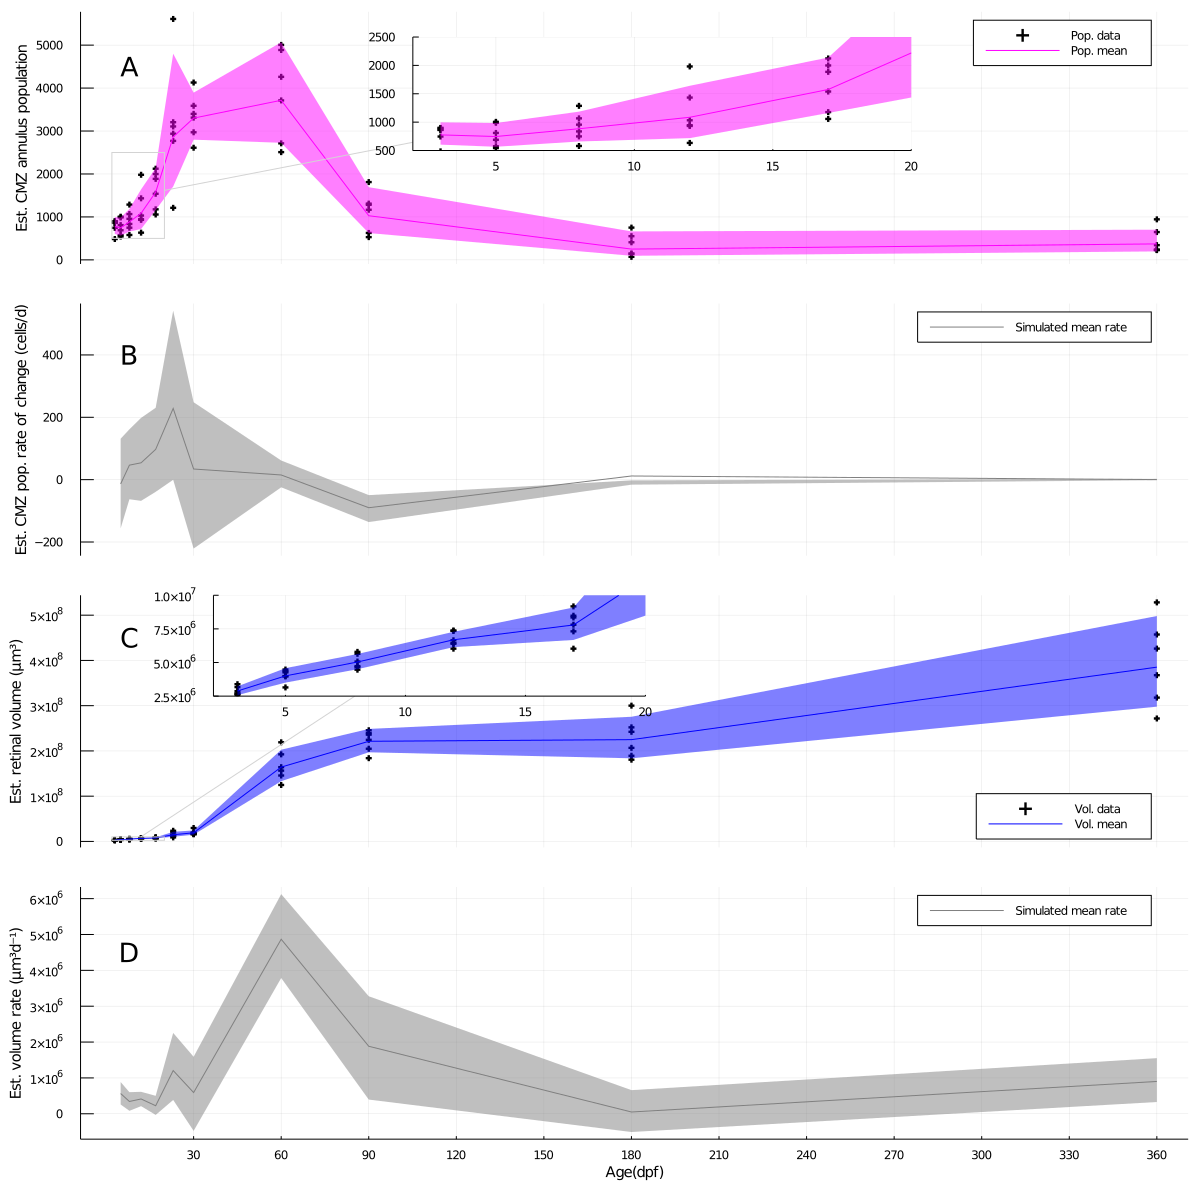
\includegraphics[width=1.\textwidth]{cmz/CMZoverall.png}}    
    \caption{{\bf Population and activity of the CMZ over the first year of \textit{D.rerio} life}}
    Panel A: Marginal posterior mean CMZ annulus population. Panel B: Marginal posterior mean retinal volume estimate. Insets in Panels A \& B display data from 3-17 dpf. Panel C: Marginal posterior mean of the proliferative index of the CMZ annulus, assayed by specified retinal neurons with incorporated thymidine from an 8hr pulse at the indicated ages. Panel D: Mean daily rate of volumetric increase of the neural retina, calculated as the difference in volumes between two ages over the number of elapsed days. All means are displayed in a band representing the $\pm 95 \%$ credible interval for the marginal posterior distribution of the mean.
    \label{CMZoverall}
    Methods in \autoref{ssec:CMZpopvolest}, \autoref{ssec:MCrates}.
    Code in \autoref{ssec:a10popsurvey}.
\end{figure}

The lack of growth observed in the first week of life suggests qn initial quiescent period in the population history of the CMZ. Observations in \autoref{rysCMZontogeny}, which demonstrate that CMZ RPCs are proliferating too slowly to be labelled by a day's pulse of a thymidine analogue at 5dpf in the wild-type and heterozygote siblings of npat mutants, also suggest this quiescence. On the other hand, we have good confidence that retinal volume continues to grow over this time; 99.56\% of the marginal posterior mass of the mean 5dpf estimate is above the 3dpf mean, which may indicate this proliferative pause is too short to appear in the retinal volume data.

In any case, the first two to three weeks of life (magnified in lens insets in panels A and C) see a relatively slow build in both estimated CMZ annulus population and retinal volume compared to the explosion which follows immediately thereafter. While zebrafish are better staged by size than age \cite{Parichy2009}, the onset of this explosive growth seems to come earlier than the typical metamorphic transition from larval to juvenile stages at ~45dpf \cite{Singleman2014}. This raises the question of how the CMZ contributes to the retina during the critical period of exponential growth of the organism, between about 45 and 90dpf. It is plausible, for instance, that the growth of the CMZ population mainly reflects the increased output of stem cells, with RPCs specifying at some steady rate, or that the CMZ builds itself up for a wave of niche exit and specification somewhat later, similarly to the sequence of events in the embryonic central retina.

In order to ascertain this timing, we simulated the mean daily rate of CMZ annulus population and retinal volume change, by performing Monte Carlo difference operations between samples from the marginal posterior means of subsequent timepoints. These simulated mean rates and their associated confidence intervals are plotted in \autoref{CMZoverall} panels B and D. These show the time-structure of the phenomenon; the increase in simulated daily CMZ population growth rate occurs before the increase in retinal volume, but the CMZ population estimate does not begin to drop off until 60dpf, by which time the majority of volumetric growth is complete. This seems to substantiate some combination of the scenarios outlined above: there is an early buildup of CMZ population around 18-30dpf, before CMZ RPCs begin to make their primary contribution to the retina between 30-60dpf, which is characterised by much slower population growth and more rapid volumetric growth, implying steady and elevated specification and niche exit of RPCs. The greater uncertainty associated with our population estimates, relative to their magnitude, results in correspondingly less certainty about the size of the population growth rate spike. For instance, we calculate a >99\% probability that the mean retinal volumetric rate growth peak at 60 dpf is at least 6-fold greater than the mean at 30dpf. By contrast, only about 97\% of the posterior mean density of the population growth rate at the 23d peak (230.2 $\frac{cells}{d}$) is greater than the mean at 3dpf, which is a small negative value (-5.5 $\frac{cells}{d}$). 

Subsequent to the bulk of the CMZ buildup and contribution to the retina, the population of the CMZ declines at about 39\% the rate of its peak ascent, with an estimated -90.1$\frac{cells}{d}$ by 90dpf. This thins out the CMZ population to below its inital postembryogenesic size, spread out over a much larger peripheral annulus, for a much less dense mature CMZ. Interestingly, the 95\% CI on the marginal posterior mean of estimated retinal volume at 180 dpf (ranging from \SI{1.84E8}{\cubic\micro\metre} to \SI{2.75E8}{\cubic\micro\metre}) completely encompasses the 95\% CI on volume at 90dpf (\SI{1.96E8}{\cubic\micro\metre}-\SI{2.48E8}{\cubic\micro\metre}), while the 360dpf mean (\SI{3.85E8}{\cubic\micro\metre}) is greater than six standard deviations from the 180dpf mean (\SI{2.25E8}{\cubic\micro\metre}). This suggests a possible second period of quiescence from approximately 90-180dpf, followed by steady contribution to the retina without a buildup in the CMZ population subsequently.

Given this description, the ontogeny of the CMZ as a stem cell niche could be well-described by different phases of activity, with different rates of proliferation and specification. It is not immediately clear what sort of periodization is justified by the data. It seems plausible that as few as two phases could explain the data well enough: an initial phase of logarithmic growth, with short cell cycle time and lower exit rate of RPCs from the CMZ into the specified neural retina, followed by a second phase of decay with longer cycle time and higher exit rate. On the other hand, perhaps some of the data features noted above justify a more bespoke model that captures, for instance, the initial quiescent period, or the post-180dpf growth of the retina. Because this is straightforwardly a question of how much model structure is justified by our data, we may address it as a model selection problem, using the system of Bayesian inference provided by nested sampling, and it is to this we now turn.

\section{Two-phase periodization of postembryonic CMZ activity by phased difference equation modelling}
\label{sec:phaseGMC}
To perform our model selection task, we must simulate the time-evolution of CMZ population and retinal volume. This requires us to supply initial values for the size of the simulated CMZ populations and the volumes of the simulated retinae they are associated with. Given the findings presented in \autoref{gausscorrelation}, we are justified in initializing CMZ population and retinal volume by independent samples from the Log-Normal models of their interindividual variability at 3dpf, at the end of embryogenesis and the beginning of CMZ-driven retinal growth. In order to produce new, simulated values of CMZ population and retinal volume, we apply a system of difference equations as follows, where $pop_n$ is the population at $n$ dpf, $CT$ is the mean cell cycle time of the population in hours, and $\epsilon$ is the proportion of the population at time $n-1$ that exits cycle and contributes to the volume of the specified neural retina, and $\mu_{cv}$ is the mean volume per cell contributed to the retina in \si{\cubic\micro\metre}:

\begin{equation}
    p_n=p_{n-1} \cdot 2^{\frac{24}{CT}} - p_{n-1} \cdot \epsilon
    \label{popeq}
\end{equation}

\begin{equation}
    v_n=v_{n-1} + p_{n-1} \cdot \epsilon \cdot \mu_{cv}
    \label{voleq}
\end{equation}

A model "phase" can then be defined by the $CT$ and $\epsilon$ parameters it applies to update the population and volume, over the appropriate number of days. The full parameterisation of a model with $p$ phases is given by $p$ pairs of $CT$ and $\epsilon$ values, and $p-1$ phase transition times. $\mu_{cv}$, which is taken to apply equally to all phases, is estimated from 3 dpf nuclear measurements, as described in \autoref{ssec:CMZpopvolest}. Given an initial population and volume sampled from the Log-Normal models of their interindividual distributions, \autoref{popeq} and \autoref{voleq} are be applied to these values to produce simulated sample values at the times actually observed. Many such samples obtained by \hyperref[ssec:Montecarlo]{Monte Carlo} can be used to estimate Log-Normal distributions for the model parameters, which can be used to score the model against observations. By defining prior distributions over the model parameters, we may sample from the prior to initialize a model ensemble. The ensemble can then be compressed by nested sampling, moving each model-particle over the parameter space by Galilean Monte Carlo, as described in \autoref{GMC}. Using typical procedures applied in nested sampling \cite{Skilling2006}, we estimated the Bayesian evidence, maximum a posteriori, and marginal posterior distributions on parameters for 2 and 3-phase models.

\begin{figure}[!h]
    \makebox[\textwidth][c]{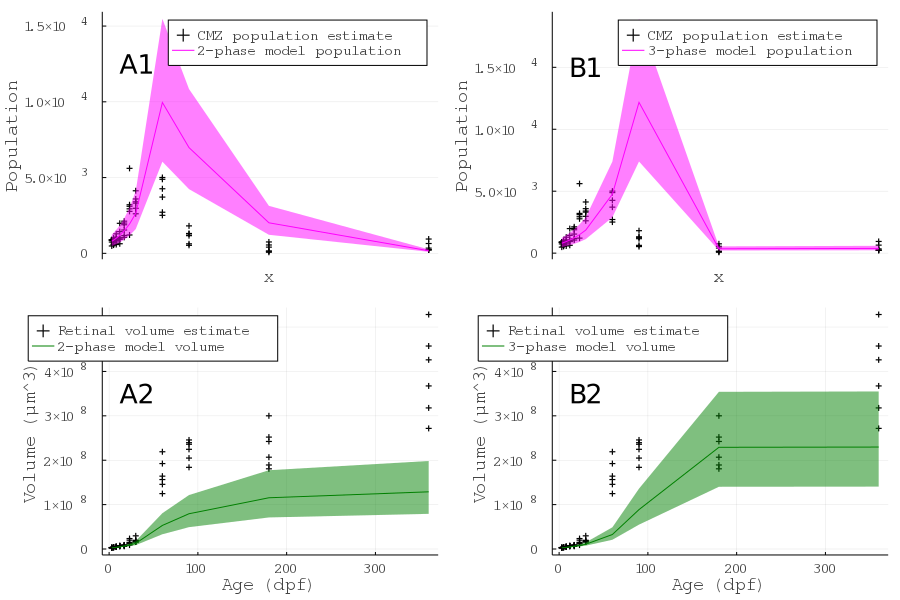
\includegraphics[width=1.2\textwidth]{cmz/a10pMAP.png}}    
    \caption{{\bf Maximum a posteriori output of periodization models}}
    \label{phaseMAPout}
    Population and volume estimates from observations (crosses) plotted with mean $\pm$ 95\% probability density model output, for the 2-phase model (A panels) and 3-phase model (B panels). A1,B1: population estimates. A2,B2: volume estimates. Insets provide magnified views of data from the first 30dpf.
    Methods in \autoref{ssec:GMCev}.
    Code in \autoref{ssec:a10periodisation}.
\end{figure}

It is useful to begin with the maximum a posteriori model output, as this shows the major problem with this simple model; the model relationship between changes in CMZ population and changes in volume breaks down after 30dpf. That is, the later volume estimates are too large for the CMZ to produce, given the calculated cellular volume ($\mu_{cv}$) at 3dpf. The models fit the early population and volume data quite well, but the population peak is dragged upward to produce more-likely volume output at later ages. While it is possible that the later CMZ contributes more volume per neuron to the cellular retina, it seems more likely that the volume approximation applies better to more-nearly spherical eyes at younger ages, than to the flattened eyes of later ages. Although we hoped that the estimated retinal volume data would constrain the $\epsilon$ exit rate parameters, this was not the case, as discussed below. When we tried floating $\mu_{cv}$ as a variable within the model, the MAP results were similar (data not shown), suggesting that a constant value for $\mu_{cv}$ across ages is the problem in achieving good model fits, not the particular value chosen. This reinforces the idea that the problem relates to the breakdown of the retinal volume estimate at later ages.

While this limitation prevents either model from explaining the combined estimate datasets very well, they are in this sense under the same constraint, and so a reasonable inference about the number of phases justified by the data is still possible. Evidence estimates for the 2-phase and 3-phase models, given these data, are presented in \autoref{phasetable}. There are greater than 3500 orders of magnitude more evidence for the 2-phase model; this result has over 200 standard deviations of significance. This reflects the expanded parameter space in the 3-phase model, which has 8 parameters, compared to the 2-phase models' 5. The additional flexibility afforded by the 3rd phase in fitting the later volume data is unable to overcome the evidentiary penalty associated with the larger parameter space. We conclude that the 2-phase hypothesis must be accepted.

\begin{table}[!ht]
    \centering
    \caption{{\bf Evidence favours a 2-phase periodization of CMZ activity}}
    \begin{tabular}{|l|l|l|l|} \hline 
        {\bf 2-phase logZ} & {\bf 3-phase logZ} & {\bf logZR} & {\bf $\sigma$ Significance}\\ \hline
        \textbf{-7147.3 ± 9.4} & -10743.0 ± 13.0 & 3596.0 ± 16.0 & 227.624\\ \hline
        \end{tabular}
    \begin{flushleft} logZ: logarithm of p(D), the marginal likelihood of the data, or model evidence. logZR: evidence ratio; positive ratios in favour of the 2-phase model. Largest evidence value bolded.
    Methods in \autoref{ssec:GMCev}.
    Code in \autoref{ssec:a10periodisation}.
    \end{flushleft}
    \label{phasetable}
\end{table}

While the parameter estimates associated with these models are clearly unreliable, they are useful to inspect in order to demonstrate some properties of nested sampling, and for comparison to the simulations to follow. To begin with, we present the parameterization of the MAP model output displayed above in \autoref{phaseMAPtable}. Unsurprisingly, the selected 2-phase model begins with a first phase of rapid proliferation, with a $CT$ of 14.5 hr, followed by a second, slower phase of 17.5 hr. The imputed exit rate $\epsilon$ is greater than 200\% of the day's starting population in the first phase, suggesting that new cells exit the CMZ after about 12 hours, around one cycle, while the second phase exit rate is lower, with 160\% of the day's starting population exiting the CMZ, again suggesting a residency time of about one cycle. The imputed phase transition age is about 23dpf. Due to the volume estimate problem noted above, it is reasonable to believe that the $CT$ estimates are likely too short, the $\epsilon$ estimates too high, all favoured in order to produce higher volume estimates at later ages.

\begin{table}[!ht]
    \centering
    \caption{{\bf Maximum a posteriori parameter estimates for periodization models}}
    \begin{tabular}{|l|l|l|}
        \hline
        {\bf Parameter} & {\bf 2-phase MAP} & {\bf 3-phase MAP}\\ \hline
        Phase 1 $CT$ (h) & 14.5 & 14.9\\ \hline\
        Phase 1 $\epsilon$ & 2.02 & 1.95\\ \hline
        Phase 2 $CT$ (h) & 17.5 & 75.6\\ \hline
        Phase 2 $\epsilon$ & 1.6 & 0.29\\ \hline
        Phase 3 $CT$ (h) & NA & 68.4\\ \hline
        Phase 3 $\epsilon$ & NA & 0.27\\ \hline
        Transition 1 age & 23.2 & 47.9\\ \hline
        Transition 2 age & NA & 179.4\\ \hline
    \end{tabular}
    \begin{flushleft}
        $CT$: cycle time.
        $\epsilon$: niche exit rate.
        Methods in \autoref{ssec:GMCev}.
        Code in \autoref{ssec:a10periodisation}.    
    \end{flushleft}
    \label{phaseMAPtable}
\end{table}

Because nested sampling naturally produces samples from the posterior, we can estimate posterior distributions using the evidence values for these samples. We performed this by kernel density estimation, specifically to investigate the extent to which the marginal posterior distributions for the selected model are polymodal; that is, the extent to which the evidence supports multiple hypotheses about the parameters of the two imputed phases. Kernel density estimates (KDEs) for marginal posterior distributions on the 2-phase models' parameters are presented in \autoref{phasemarginals}. 

These estimates reveal monomodal posterior distributions over the parameters. $CT$ posteriors are well constrained to a small part of the sampling space (left panels, X axes, and top right panel), with the MAP parameter estimates given in \autoref{phaseMAPtable} falling within the most dense regions. However, it is evident that the data do not constrain phase exit rates $\epsilon$ (left panels, Y axes) very well. That is, the marginal posterior probability distributions for these parameters are very widely spread.  The marginal posterior distribution on the age at which the transition between phases occurs is plotted in the bottom right of \autoref{phasemarginals}; the KDE suggests that the age of phase transition must be around 23 dpf.

\begin{figure}[!h]
    \makebox[\textwidth][c]{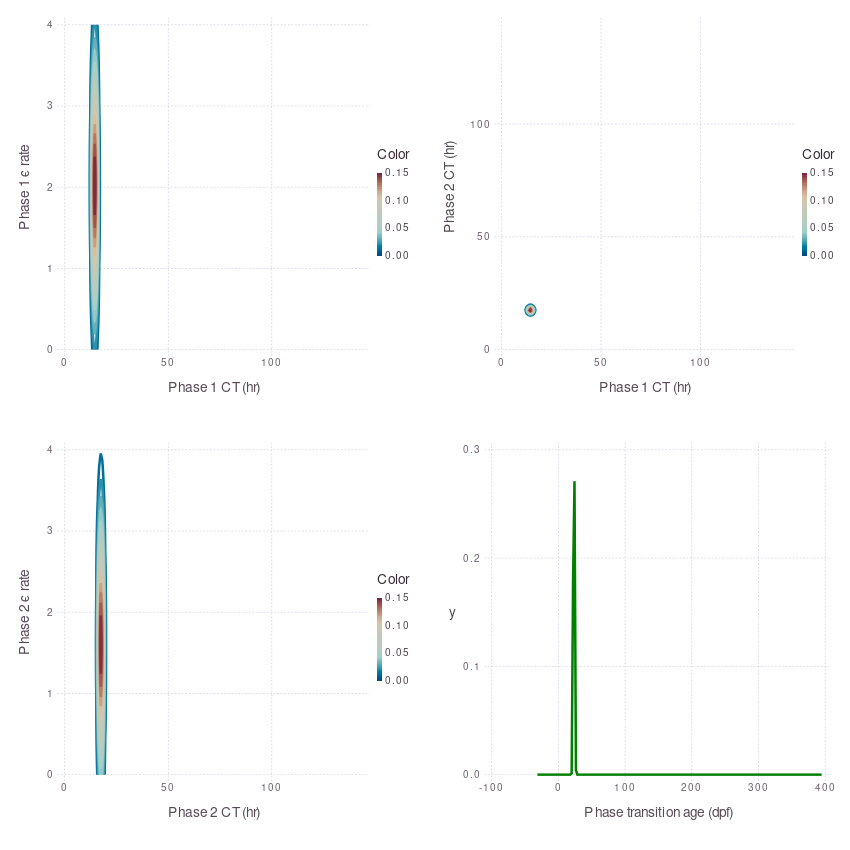
\includegraphics[width=1.\textwidth]{cmz/a10pmarginals.png}}    
    \caption{{\bf Kernel density estimates of marginal posterior parameter distributions, 2-phase model}}
    Prior distributions (magenta) apply to parameters of both phases. Maximum a posteriori model parameterisation indicated by vertical lines.
    Panel A: Marginal posterior distributions on Phase 1 and 2 $CT$ cycle time parameters. 
    Panel B: Marginal posterior distributions on Phase 1 and 2 $\epsilon$ niche exit rate parameters.
    Panel C: Marginal posterior distribution on Phase 1 to 2 transition age parameter.
    \label{phasemarginals}
    Methods in \autoref{ssec:GMCkde}.
    Code in \autoref{ssec:a10periodisation}.    
\end{figure}

We conclude that, while our global model of CMZ population and volumetric retinal contribution is too flawed to make good parameter estimates, a 2-phase model of this activity is far better substantiated by the evidence than a 3-phase model. We proceed on this basis, accepting the 2-phase model, and taking up the idea of the "slice model" introduced in \autoref{ssec:slice}, to investigate modelling the CMZ RPC population more concretely, directly from sectional observations, rather than from the calculated population and retinal volume estimates presented above.

\FloatBarrier

\section{Slice-model characterisation of asymmetrical CMZ population dynamics demonstrates anatomical homogeneity of proliferative schedule}
\label{sec:sliceGMC}

In the course of the preceding investigations, it became apparent that the CMZ population asymmetry mentioned in \autoref{chap:SMMEoutro} was not a static phenomenon, with the dorsal lobe of the CMZ annulus being consistently more populous than the ventral lobe, as generally implied by the sources covered in \autoref{chap:RPCreview}. Rather, both the extent and orientation of asymmetry seem to evolve over time. Sectional population totals for the dorsal and ventral CMZ are presented in \autoref{DVontology}, Panel A, alongside the related intra-individual asymmetry ratio in Panel B. The initially pronounced dorsal population and reduced ventral population both seem to go through the overall boom-bust progression of CMZ population, but their relative proportion within individuals reverses itself over the period from 17-90dpf. We also observed a similar phenomenon occurring across the naso-temporal axis over the same time period (\autoref{NTontology}).

\begin{figure}[!h]
    \makebox[\textwidth][c]{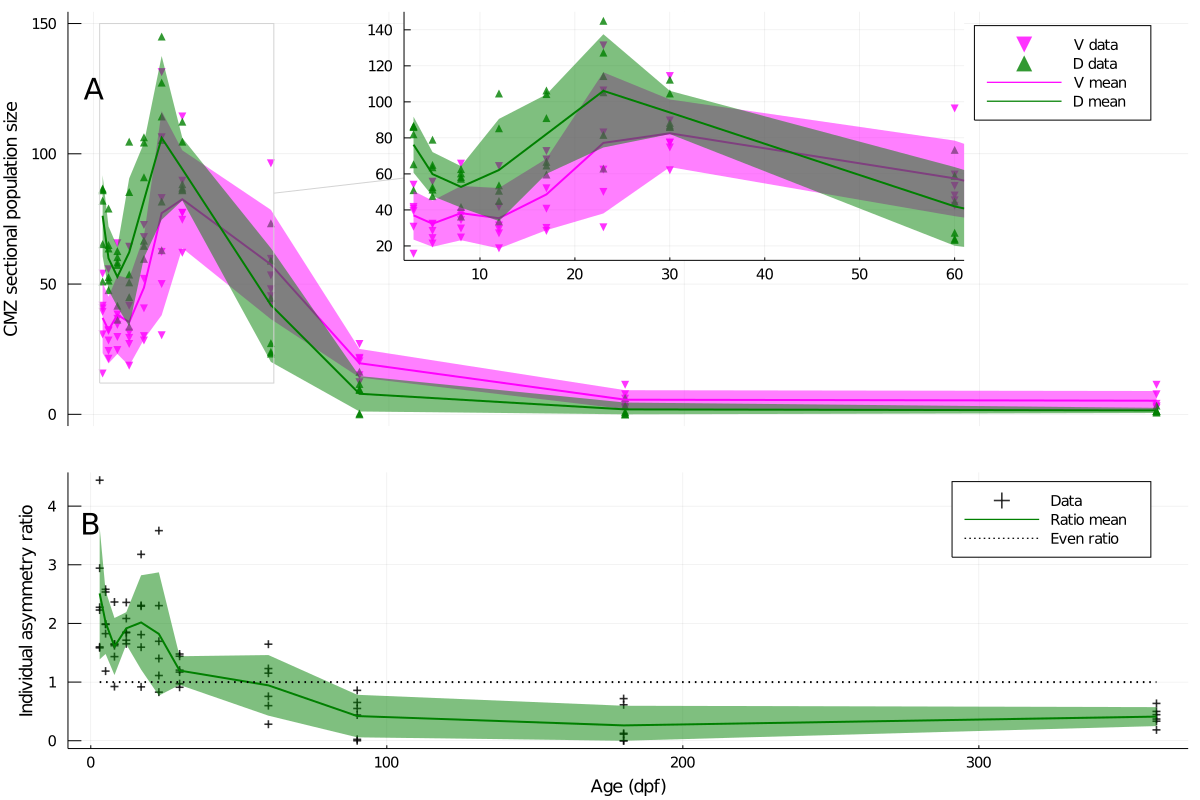
\includegraphics[width=1.2\textwidth]{cmz/DVontology.png}}    
    \caption{{\bf Developmental progression of dorso-ventral population asymmetry in the CMZ.}}
    Marginal posterior distribution of mean dorsal (D) and ventral (V) population size in 14$\mu$m coronal cryosections (panel A) or intra-individual D/V count asymmetry ratio (panel B), $\pm 95\%$ credible interval, n=5 animals per age. Data points represent mean counts from three central sections of an experimental animal's eye. 
    \label{DVontology}
    Methods in \autoref{ssec:PCNA}.
    Code in \autoref{ssec:a10dvratio}. 
\end{figure}

Inspected closely, these data provide a possible rationale for the reversal of asymmetry in the proliferative dynamics of the niche itself: the sectional (or ``slice'') population of the dorsal CMZ is increasing beyond its postembryonic minimum by 12dpf, while the ventral CMZ takes until 17dpf to exhibit a noticeable increase in size; moreover, the peak dorsal population is achieved by 23dpf, whilst ventrally the peak is only achieved at 30dpf. This suggests that the dorsal and ventral CMZ populations undergo similar, time-shifted processes of proliferation from different starting populations. If this is so, an explanation for this time-shifted phenomenon could have fundamental relevance to predicting and controlling the proliferative behaviour of peripheral RPCs and stem cells.

To test this hypothesis, we used a ``slice model'' of the CMZ, where the thickness of the slice is taken to be the same as the observed cryosection thickness (\SI{14}{\micro\metre}). The population of the CMZ is modelled with a difference equation, as above, but with an additional exit term representing lateral, circumferential contributions of the CMZ to the generation of new, adjacent ``slices''. The value of this term is calculated from the difference in CMZ annulus diameter over the calculated time period, as implied by a power-law model of lens growth fitted to observations, discussed in \autoref{sec:lenspopest}. The resultant difference equation is \autoref{sliceeq}. Terms are as defined above, except that $p_n$ is the sectional population at $n$ dpf, and not the total CMZ annulus population; additionally, $\eta$ is defined as the daily circumferential exit rate implied by the power-law model.

\begin{equation}
    p_n=p_{n-1} \cdot 2^{\frac{24}{CT}} - p_{n-1} \cdot \epsilon - \eta
    \label{sliceeq}
\end{equation}

We reasoned that, if the phase transition occurs earlier in the dorsal CMZ than in the ventral CMZ, there should be some informational gain in separating these observations vs. a combined total sum for both lobes of the slice annulus\footnote{The ``total'' model is required to supply double the circumferential exit rate of the dorsal or ventral models, to reflect the requirement for this ``full'' slice to grow both lobes of the eye}. In this case, the combination of two phase-shifted populations in the total model should produce a ``fuzzy'' peak relative to the separate modes. We therefore estimated the evidence, MAP, and posterior marginals for 2-phase models given the sectional sum, dorsal, and ventral populations. To focus on the most informative subset of the data for our hypothesis, we restricted this analysis to the population data within the first three months of life.

The slice model proves to have much greater success at explaining sectional counts than the whole-eye model does at explaining the annulus population estimates; maximum a posteriori model output is presented in \autoref{dvMAPout}. In particular, all of the models adequately represent the early decline in sectional populations, arising from rapid early growth of the eye that exceeds the CMZs' proliferative capacity, without further ado; there is no justification for the early quiescent period suggested above.

\begin{figure}[!h]
    \makebox[\textwidth][c]{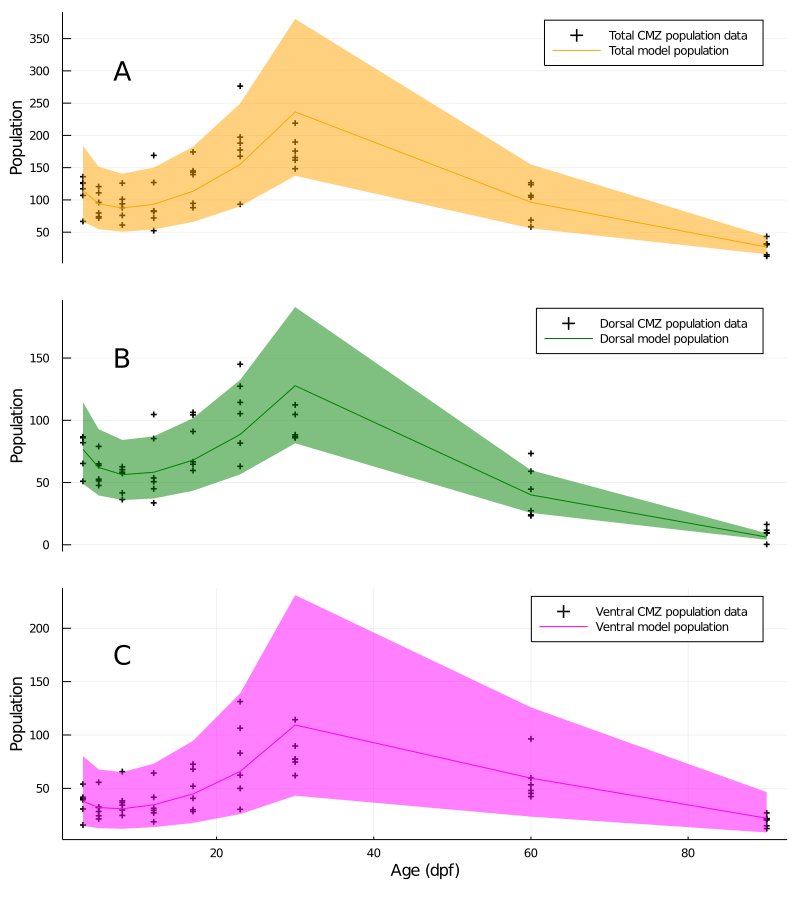
\includegraphics[width=1.0\textwidth]{cmz/a10dvMAP.png}}    
    \caption{{\bf Maximum a posteriori output of total, dorsal, and ventral CMZ slice models}}
    \label{dvMAPout}
    Population and volume estimates from observations (crosses) plotted with mean $\pm$ 95\% probability density model output, for the total CMZ population model (panel A), dorsal CMZ population model (panel B), and ventral CMZ population model (panel C).
    Methods in \autoref{ssec:GMCev}.
    Code in \autoref{ssec:a10dvslice}. 
\end{figure}

The hypothesis that there is a time-shift in the phase transition across the dorso-ventral axis is thoroughly refuted by these models, in two ways. First, the evidence estimates demonstrate that we are not justified in separating the dorsal and ventral populations. The total-population slice model receives greater than 500 orders of magnitude more evidence than the joint evidence for the separate dorsal and ventral models, with greater than 180 standard deviations of significance, as displayed in \autoref{dvtable}. It is interesting to note that the evidence for the dorsal model (
-673.5 ± 1.9) is substantially less than for the ventral model (-405.4 ± 1.2). This may indicate a causal influence on the dorsal population that is neither in the model nor acting on the ventral population, or it may be an uninformative sampling effect. 

\begin{table}[!ht]
    \centering
    \caption{{\bf Evidence favours a combined slice model over separate dorsal and ventral models}}
    \begin{tabular}{|l|l|l|l|l|}
        \hline
        {\bf Combined D/V model logZ} & {\bf Separate D/V model logZ} & {\bf logZR} & {\bf $\sigma$ Significance}\\ \hline
        \textbf{-1019.31 ± 0.86} & -1078.9 ± 2.3 & 59.6 ± 2.4 & 24.5\\ \hline
        \end{tabular}
    \begin{flushleft} logZ: logarithm of p(D), the marginal likelihood of the data, or model evidence. logZR: evidence ratio; positive ratio in favour of the combined model. Largest evidence value bolded.
    Methods in \autoref{ssec:GMCev}.
    Code in \autoref{ssec:a10dvslice}.     
    \end{flushleft}
    \label{dvtable}
\end{table}

A second indication that this hypothesis is unsupported are the MAP model parameter values, summarized in \autoref{dvMAPtable}. The MAP phase transition age for the total slice model is functionally identical\footnote{That is, both values round to 36 days in the likelihood function, which uses the discrete difference equation, with a step size of 1dpf, as indicated above.} to that for the ventral model, and within two days of the MAP transition for the dorsal model. Additionally, the dorsal MAP transition is actually later than the ventral date, which further suggests the original model-idea of a time-shifted late ventral phase change is unsupported by these data.

The MAP parameters for the total slice model confirm our supposition that those found for the 2-phase MAP in \autoref{phasemarginals} overstate cell cycle speed and exit rate. The total slice model gives $CT$s of 24.2 and 25.1 hours for the first and second phases, compared to 14.5 and 17.5 estimated previously. Moreover, the niche exit rates $\epsilon$ are estimated at .91 and .98 for the total slice model, compared to 2.02 and 1.6 for the 2-phase model. The values estimated for the slice model are likely to be more realistic, and suggest that the overall magnitude of the changes between phases is subtle. Interestingly, the MAP phase parameters differ markedly between the split dorsal\/ventral models and the total slice model. Surprisingly, the dorsal estimates suggest a faster $CT$ for the second phase. This may indicate that additional noise incurred from splitting the sectional CMZ population into dorsal and ventral lobes has a strong effect on parameter estimates. This may provide a practical reason to prefer combining these counts in slice models, beyond the calculations presented here. 

\begin{table}[!ht]
    \centering
    \caption{{\bf Maximum a posteriori parameter estimates for slice models}}
    \begin{tabular}{|l|l|l|l|}
        \hline
        {\bf Parameter} & {\bf Total MAP} & {\bf Dorsal MAP} & {\bf Ventral MAP}\\ \hline
        Phase 1 $CT$ (h) & 20.8 & 30.5 & 19.7\\ \hline
        Phase 1 $\epsilon$ & 1.14 & 0.65 & 1.23\\ \hline
        Phase 2 $CT$ (h) & 24.9 & 19.5 & 30.1\\ \hline
        Phase 2 $\epsilon$ & 1.0 & 1.4 & 0.76\\ \hline
        Transition age & 35.9 & 37.7 & 36.0\\ \hline
        \end{tabular}
    \begin{flushleft}
        $CT$: cycle time.
        $\epsilon$: niche exit rate.
        Methods in \autoref{ssec:GMCev}.
        Code in \autoref{ssec:a10dvslice}.    
    \end{flushleft}
    \label{dvMAPtable}
\end{table}

The marginal posterior distributions of the total slice model, presented in \autoref{dvmarginals}, are substantially more polymodal than those in \autoref{phasemarginals}. This illustrates how data can support multiple hypotheses about model parameters to different degrees. Exit rate $\epsilon$ posteriors are no less constrained than the whole-eye model, suggesting the retinal volume estimate supplies little additional information on the rate at which RPCs leave the niche. However, the marginal posteriors on cycle length $CT$ are less constrained than the whole-eye model, so the volume estimate may nonetheless narrow the range of credible $CT$ values. This may be a rationale for pursuing better volumetric estimates for retinae from fish older than 30 dpf. The posterior distribution on the age of phase transition indicates that many values for this parameter retain some credibility. The MAP estimate does not occupy the most probable KDE kernel for this value. An important property of nested sampling is that the accuracy of evidence calculations is traded off against the accuracy of estimating the posterior distribution, as noted in \autoref{ssec:GMC}. Since we have here prioritized evidence estimation, this is the cause of this discrepancy; the MAP models themselves have relatively little weight in the KDE estimates.

\begin{figure}[!h]
    \makebox[\textwidth][c]{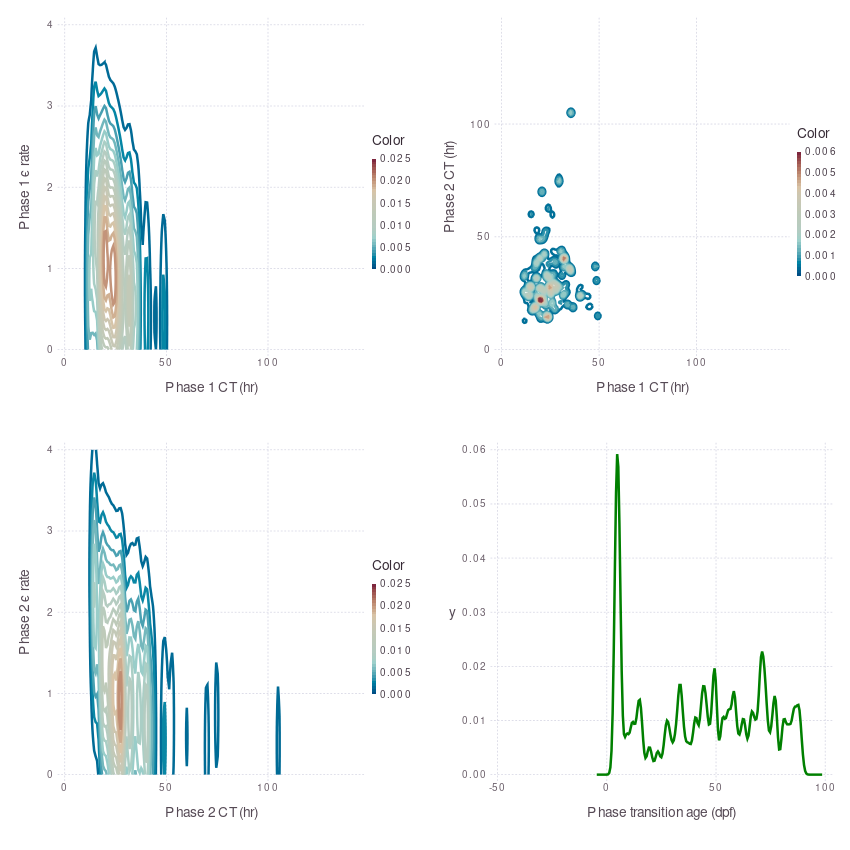
\includegraphics[width=1.\textwidth]{cmz/a10dvmarginals.png}}    
    \caption{{\bf Kernel density estimates of marginal posterior parameter distributions, total slice model}}
    Line height (bottom right panels) or color (other panels) indicates the estimated marginal posterior mass present at the indicated parameter value.
    Top left panel: Phase 1 $\epsilon$ exit rate vs Phase 1 $CT$ cycle time (hr).
    Bottom left panel: Phase 2 $\epsilon$ exit rate vs Phase 2 $CT$ cycle time (hr).
    Top right panel: Phase 2 $CT$ cycle time (hr) vs Phase 1 $CT$ cycle time (hr).
    Bottom right panel: Estimated marginal posterior mass vs. phase transition age (dpf)
    \label{dvmarginals}
    Methods in \autoref{ssec:GMCkde}.
    Code in \autoref{ssec:a10dvslice}.    
\end{figure}

On the basis of this analysis, the best available hypothesis about the observed ontogeny of RPC population asymmetry across the dorsoventral axis is the pre-establishment of differential population size by asymmetrical progress of the embryonic specification wave, rather than differential proliferative schedules.

\FloatBarrier

\subsection{Cumulative thymidine labelling supports Galilean Monte Carlo Nested Sampling inference}
\label{ssec:CMZcumedu}

To investigate the accuracy of the parameter estimates provided by the model studies above, we sought to confirm their plausibility by examining 3dpf CMZ RPCs cumulatively labelled with a 10.5 hour pulse of the thymidine analogue EdU. We used the Empirical Bayes approach to estimate the evidence for separate Nowakowski-style \cite{Nowakowski1989} linear models for the dorsal and ventral CMZ, against a model for both subpopulations combined. While this model is inadequate for reasons described in \autoref{sec:Nowakowski}, it can serve to substantiate the first phase cycle time parameter. These results are summarized in \autoref{cumEdUtable}, with the relevant linear regressions displayed in Supplementary \autoref{cumEdUlinreg}.

\begin{table}[!ht]
    \centering
    \caption{{\bf Evidence favours whole-CMZ linear cycle models over separate D/V models}}
    \begin{tabular}{|l|l|l|l|} 
        \hline {\bf Model} & {\bf Implied $T_c$ (hr)} & {\bf Implied $T_s$ (hr)} & {\bf logZ}\\ \hline 
        Dorsal & 14.7 $\pm$ 1.6 & 1.38 $\pm$ 0.76 & 7.778\\ \hline 
        Ventral & 14.0 $\pm$ 1.2 & 0.8 $\pm$ 0.58 & 15.202\\ \hline
        Combined & 14.6 $\pm$ 1.1 & 1.25 $\pm$ 0.53 & {\bf26.165}\\ \hline
    \end{tabular}
   
    \begin{flushleft} $T_c$: calculated cell cycle time. $T_s$: calculated s-phase length. logZ: logarithm of p(D), the marginal likelihood of the data, or model evidence.  Largest evidence value bolded.
    Methods in \autoref{ssec:CMZEmpBayes}.
    Code in \autoref{ssec:a25dvlinreg}.    

    \end{flushleft}
    \label{cumEdUtable}
\end{table}

Firstly, there are approximately 3 orders of magnitude of evidence in favour of the combined model vs. the joint evidence for separate models (ie. 26.165 vs. 22.980). This model provides no support for differing cell cycle characteristics across the D/V retinal axis of asymmetry at 3dpf. This confirms that the differing D/V MAP parameter estimates observed in the slice model are unsubstantiated; the evidence supports broadly similar cell cycle characteristics across anatomical axes in 3dpf CMZ RPCs. The Nowakowski-calculated cell cycle time $T_c$ for the combined model, 14.6 $\pm$ 1.1 hr, includes the whole-eye MAP first phase $TC$, 14.5 hr, within one standard deviation, although not the first phase $TC$, 24.2 hr. This suggests the Nowakowski model has similar problems to the whole-eye models presented in \autoref{phaseMAPout}, substantially overstating cycle rate. Calculated S phase lengths are also unrealistically short. Finally, the data clearly diverge from a linear trend toward the end of the pulse (see \autoref{cumEdUlinreg}), showing the limitations of this model.

\begin{figure}[!h]
    \makebox[\textwidth][c]{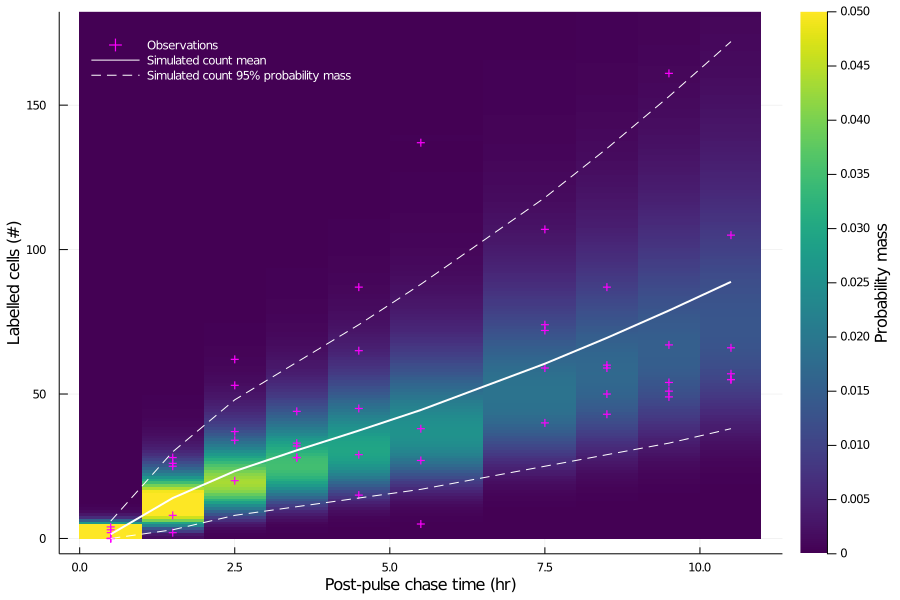
\includegraphics[width=1.\textwidth]{cmz/a25MAP.png}}    
    \caption{{\bf MAP model output and observations for thymidine slice model of 3dpf cumulative EdU labelling}}
    Count of EdU-positive cells observed in 14\si{\micro\metre} coronal cryosections through \textit{Danio} CMZs, at indicated chase times, during a 10 mM EdU pulse (magenta crosses), overlaid with MAP model output. Probability mass distribution of the discrete non-parametric output is shown by color scale; yellow values include counts with >.05 mass. Output mean and 95\% mass are indicated by solid and dashed white lines.

    Methods in \autoref{ssec:rysBrdUpulse}.
    \label{a25MAP}
\end{figure}

\begin{figure}[!h]
    \makebox[\textwidth][c]{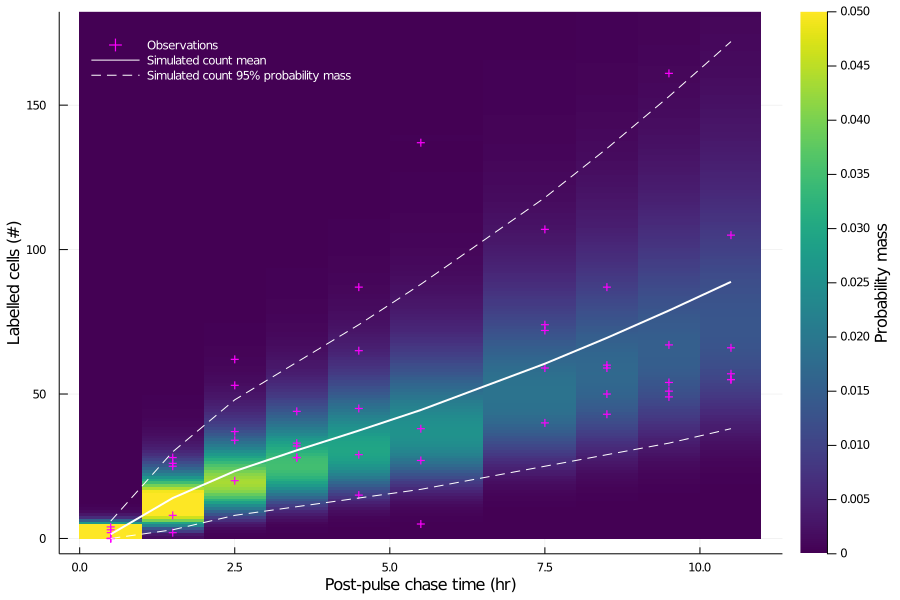
\includegraphics[width=1.\textwidth]{cmz/a25MAP.png}}    
    \caption{{\bf MAP model output and observations for thymidine slice model of 3dpf cumulative EdU labelling}}
    Count of EdU-positive cells observed in 14\si{\micro\metre} coronal cryosections through \textit{Danio} CMZs, at indicated chase times, during a 10 mM EdU pulse (magenta crosses), overlaid with MAP model output. Probability mass distribution of the discrete non-parametric output is shown by color scale; yellow values include counts with >.05 mass. Output mean and 95\% mass are indicated by solid and dashed white lines.

    Methods in \autoref{ssec:rysBrdUpulse}.
    \label{a25MAP}
\end{figure}

\begin{figure}[!h]
    \makebox[\textwidth][c]{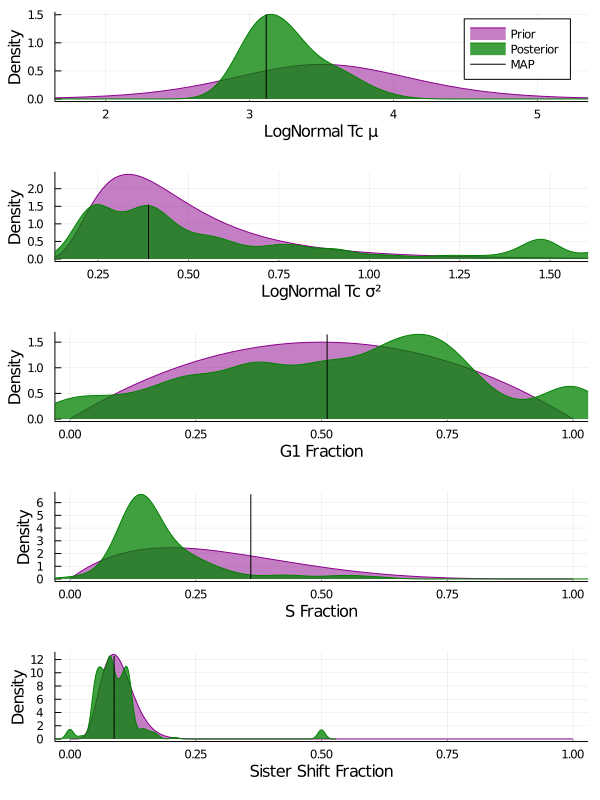
\includegraphics[width=1.\textwidth]{cmz/a25marginals.png}}    
    \caption{{\bf MAP model output and observations for thymidine slice model of 3dpf cumulative EdU labelling}}
    Count of EdU-positive cells observed in 14\si{\micro\metre} coronal cryosections through \textit{Danio} CMZs, at indicated chase times, during a 10 mM EdU pulse (magenta crosses), overlaid with MAP model output. Probability mass distribution of the discrete non-parametric output is shown by color scale; yellow values include counts with >.05 mass. Output mean and 95\% mass are indicated by solid and dashed white lines.

    Methods in \autoref{ssec:rysBrdUpulse}.
    \label{a25marginals}
\end{figure}

\section{The CMZ contributes stably to each cellular layer with time-variable lineage composition}

By labelling CMZ RPCs with the thymidine analogue EdU in a pulse at 3, 23, and 90 dpf, followed by histochemical analysis for known zebrafish retinal neural lineage markers after a 7 day chase, we investigated the possibility that RPC lineage outcomes change over the life of the organism. This hypothesis is of particular interest, as differences in the mosaic organisation of embryonically-contributed central retina and CMZ-contributed peripheral retina remain unexplained \cite{Allison2010}. It may, moreover, have clinical significance, were quiescent peripheral stem cells to be entrained for regnerative medical purposes, as their lineage outcomes may be different than embryonic RPCs.  We used antibodies raised against Pax6 and Isl2b to mark retinal ganglion cells (RGCs) of the ganglion cell layer and amacrine cells of the inner nuclear layer. Anti-glutamine synthetase (GS) and anti-PKC$\beta$ were used to mark M\"{u}ller glia (MG) and bipolar cell (BPC) populations of the INL. The unique flattened nuclear morphology of horizontal neurons was used to identify them. Lastly, the antibody Zpr1, directed against an unknown antigen present in photoreceptors with double cone morphology, was used to mark these cells.

\begin{figure}[!h]
    \makebox[\textwidth][c]{\includegraphics[width=1.2\textwidth]{cmz/lineage.png}}    
    \caption{{\bf Representative 23dpf lineage marker confocal micrographs}}
    Panel A1: RGC/Amacrine staining group. A2: Isl2b channel. A3: Pax6 channel.

    Panel B1: MG/BPC staining group. B2: PKC$\beta$ channel. B3: GS channel.

    Panel C: Double cone staining group. Zpr1 channel.

    GCL: Ganglion cell layer. INL: Inner nuclear layer. ONL: Outer nuclear layer.
    Methods in \autoref{CMZlintrace}.
    \label{staininggroups}
\end{figure}

Observations were collected in "staining groups", which combined histological markers; representative confocal micrographs from this study in animals pulsed at 23dpf are displayed in \autoref{staininggroups}, while data from all ages are plotted in \autoref{layercontributions}. It is worth noting that the relative position of the CMZ-contributed cohort is very different in older animals, with 7 days of chase time being just enough for the majority of the 90dpf cohort to be reliably located within the specified neural retina, as depicted in supplementary \autoref{90dpfcohort}. Because we suspect that CMZ-contributed retinal cohorts may be subject to a process of attrition, and that this turnover might be higher near the CMZ, as discussed in \autoref{sec:neuralfate}, if this hypothetical turnover process has differential effects over time on specified retinal neurons of different lineages, results may not be directly comparable between ages. With that caveat, we proceed to the lineage data.

\begin{figure}[!h]
    \makebox[\textwidth][c]{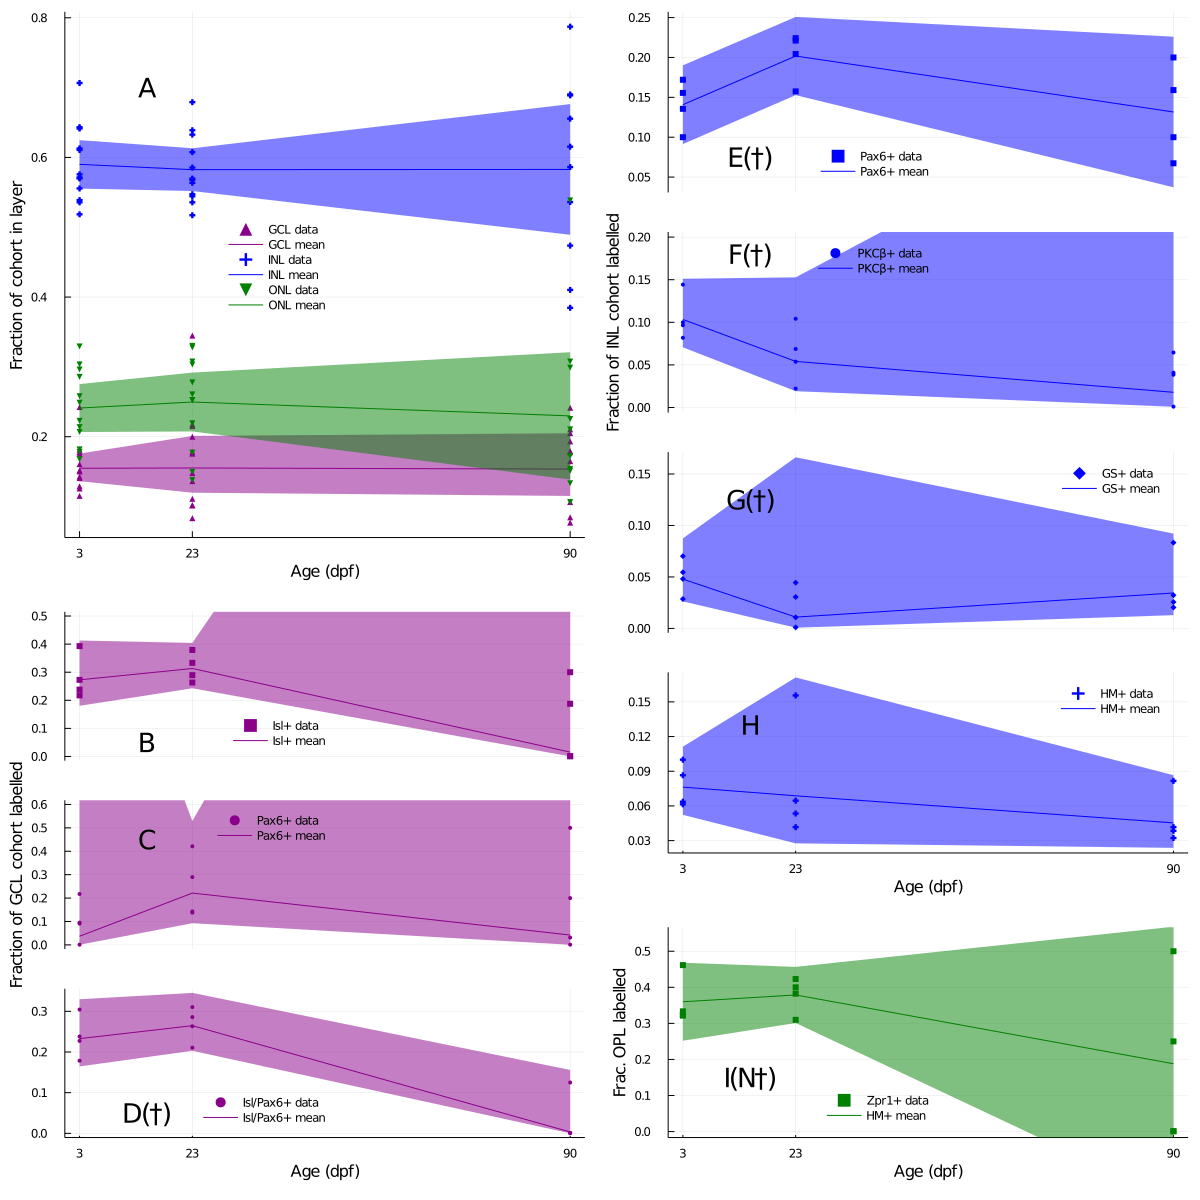
\includegraphics[width=1.2\textwidth]{cmz/layercontributions.png}}    
    \caption{{\bf Second-phase declines in CMZ-contributed Isl\/Pax6+ RGCs, PKC$\beta$+ bipolar neurons, and Zpr1+ double cones}}
    Overall fraction of CMZ-contributed cohort entering cellular layers (Panel A), or fraction of the layer subcohort expressing the noted immunohistochemical marker of lineage. All mean values are presented as marginal posterior means $\pm$ 95\%CI.

    $\lambda$: Fractional lineage contribution is modelled Log-Normally

    $\dagger$: Evidence supports time-varying model of fractional lineage contribution

    Magenta: GCL measurements; Blue: INL measurements; Green: ONL measurements

    Methods in \autoref{ssec:CMZlintrace}, \autoref{ssec:GMCev}.
    Code in \autoref{ssec:a19lineagetrace}.    
    \label{layercontributions}
\end{figure}

These data take the form of fractions of the thymidine-labelled cohort entering each of the three cellular layers (panel A of \autoref{layercontributions}), or the subfraction of the cohort within a given layer expressing a particular cellular marker (Panels B-I). While some variability is apparent in all of the measurements, it is unclear whether it is well-described as time-dependent in most cases. In order to address the question of whether CMZ layer or lineage outcomes differ over time, we needed to assess the joint evidence for separate models of each measurement at each age, against the evidence for a single model of the measurement for all of the assessed ages. 

Because it is not obvious that these fractional measurements are better described Log-Normally as the underlying population counts are, we first assessed the joint evidence for Normal and Log-Normal models of the data, summarized in Supplementary \autoref{lineage_nlnev}. Our evidence supports Log-Normal modelling of all measurements aside from the INL and ONL, as well as INL-resident Pax6- and ONL-resident Zpr1-positive cells. We noted that the evidence estimates confirmed simple likelihood ratio tests in most cases, as summarized in Supplementary \autoref{lineage_lhratio}, with only INL totals, GS+, ONL total, and Zpr1+ results disagreeing with the evidence estimates. This demonstrates a case where full evidence estimation can produce differing results from maximum likelihood methods for multiple measurements.  Without a clear fundamental justification for uniformly preferring one model or the other, we selected the best-supported model for each measurement. We estimated the evidence for an age-marginalized model, representing stable contribution to the layer or lineage over time, and compared this to the joint evidence for separate models at each age, representing a time-varying contribution model. These estimates are presented in \autoref{lineage_ev}.

\begin{table}[!ht]
    \caption{{\bf Evidence supports stable layer contributions with time-varying lineage contributions}}
    \begin{tabular}{|l|l|l|l|l|l|l|} 
        \hline
        {\bf Layer} & {\bf Marker} & {\bf Cell type} & {\bf Stable logZ} & {\bf Time-vary logZ} & {\bf logZR} & {\bf $\sigma$ sign.}\\ \hline \hline
        GCL & Cohort & All GCL cells & {\bf -53.473 ± 0.055} & -63.93 ± 0.19 & 10.46 ± 0.2 & 52.8\\ \hline \hline
        GCL & Isl2b & RGC & {\bf -54.58 ± 0.9} & -56.3 ± 0.76 & 1.7 ± 1.2 & 1.4\\ \hline
        GCL & Pax6 & Displaced am. & {\bf -31.09 ± 0.12} & -35.39 ± 0.34 & 4.3 ± 0.36 & 12.0\\ \hline
        GCL & Isl2b/Pax6 & RGC subtype & -43.76 ± 0.76 & {\bf -16.38 ± 0.18} & -27.37 ± 0.78 & 34.9\\ \hline \hline
        INL & Cohort & All INL cells & -131.4 ± 1.4 & {\bf -84.56 ± 0.91} & -46.9 ± 1.7 & 27.8\\ \hline \hline
        INL & Pax6 & Amacrine cell & -15.8 ± 0.024 & {\bf -13.99 ± 0.24} & -1.81 ± 0.24 & 7.5\\ \hline
        INL & PKC$\beta$ & Bipolar cell & -3.86 ± 0.2 & {\bf 8.68 ± 0.44} & -12.54 ± 0.48 & 26.0\\ \hline
        INL & GS & M\"{u}ller glia & 15.78 ± 0.25 & {\bf 14.18 ± 0.48} & 1.6 ± 0.54 & 3.0\\ \hline
        INL & HM & Horizontal cell & {\bf 10.79 ± 0.41} & 9.15 ± 0.37 & 1.65 ± 0.55 & 3.0\\ \hline \hline
        ONL & Cohort & All ONL cells & {\bf -79.87 ± 0.97} & -128.68 ± 1.0 & 48.8 ± 1.4 & 35.1\\ \hline \hline
        ONL & Zpr1 & Double cones & -54.66 ± 0.92 & {\bf -42.25 ± 0.72} & -12.4 ± 1.2 & 10.6\\ \hline
    \end{tabular}
   
    \begin{flushleft}logZ: logarithm of p(D), the marginal likelihood of the data, or model evidence.  Largest evidence values bolded. logZR: evidence ratio; positive values in favour of stable model.
    Methods in \autoref{ssec:CMZlintrace}, \autoref{ssec:GMCev}.
    Code in \autoref{ssec:a19lineagetrace}.    
    \end{flushleft}
    \label{lineage_ev}
\end{table}

These calculations demonstrate that there is evidence for time-varying contributions to the retina, in particular to the INL overall, and to amacrine, bipolar, and M{\"u}ller glial fates.  Additionally, time-varying models of Isl/Pax6+ RGCs in the GCL, and Zpr1+ double cones of the ONL are all well-supported. All of these findings have between 3 and 35 standard deviations of significance. In the INL, the trend of the posterior mean for PKC$\beta$-positive bipolar neurons (panel Fand GS-positive M{\"u}ller glia of these lineages declines from the early postembryonic period (3dpf) to the late juvenile period (90dpf). Mean GCL Isl/Pax6-positive RGCs and ONL Zpr1-positive double cones also trend downward. By contrast, the posterior mean for Pax6-positive amacrine cells increases before declining. The trend of mean INL contributions is constant over this period, but variability increases markedly at 90dpf, justifying the time-varying model. These results show that CMZ RPCs do not contribute lineages in stereotypical proportions throughout the organism's lifetime; in fact, the proportions of particular lineages change over time, and contributions to the INL in particular become more variable. Since there are declining lineages in each of the three retinal layers, these lineages may be functionally related. However, we have no specific evidence that would implicate Isl2b/Pax6 double-positive RGCs in circuits with bipolar cells or double cones, for instance. In any case, this provides an explanation for the observation of a more-ordered retinal mosaic in later retinal contributions relative to the embryonic central remnant: since one or more sublineages in each layer are depleted in older fish, a different overall mosaic pattern as the neurons associate and pack together is expected. Based on the timing of these changes, we tentatively ascribe this differential lineage production to the second phase of CMZ contribution in our periodisation; the data do not have enough ime resolution to test this with more precision.

Lastly, we investigated the possibility that there might be detectable differences in layer or lineage contributions across the dorso-ventral axis; we tested this by measuring the evidence for age-marginalized combined models of fractional contribution against age-marginalized models split along the dorso-ventral axis. We found no evidence to support this hypothesis. These results are presented in Summary \autoref{lineage_dvev}.

\FloatBarrier

\section{Early retinal cohorts of the \textit{D. rerio} retina are turned over at a low rate by 4C4-positive microglia}
\label{sec:neuralfate}
Recently, extensive neural death has been reported in older zebrafish retinae \cite{Vanhoucke2018}. This was described as a ``neurodegenerative pathology" and suggested as a model of age-related neurodegeneration. However, during our thymidine analogue pulse-chase studies, CMZ-contributed cohorts often appeared less numerous only a month or two after their entry into the neural retina, even in juveniles of 30-90 days of age. Moreover, we observed numerous 4C4-positive microglia associating with the CMZ, as displayed in Supplementary \autoref{4C4overview}, which suggested that microglia may prune CMZ contributions. If neural retinal turnover occurs throughout the life of the organism, this would belie view that it should be treated as pathological, rather than constitutive. However, the thinning phenomenon could be explained by the changing morphology and geometry of the neural retina during this period. In particular, the neural retina thickens noticeably over this time, as displayed in Supplementary \autoref{morphology}. Although this increase is due, in large part, to the lengthening of photoreceptor outer segments, the inner nuclear layer is also significantly thickened. It is plausible that this process involves a compaction of the neurons along the coronal axis typically sampled, thus appearing to lose cells over time without this actually occurring. 

In order to investigate this phenomenon, we administered 24 hr pulses of EdU to 1dpf embryos, and followed with 24 hr pulses of BrdU at 23dpf to mark a CMZ-contributed cohort near the height of its activity. By taking both coronal and transverse sections through animals at 30, 60, and 90 dpf, we sampled these cohorts from both morphological axes of the retina and counted labelled sectional totals. Data from the axes were combined to account for the possibility of the cohorts being compacted on the coronal plane and extended on the transverse one. In order to test the hypothesis of early turnover, we estimated the evidence for linearly correlated and uncorrelated models of cohort population over time, using the \hyperref[empiricalBayes]{Empirical Bayes} regression method. In effect, we suppose that if the addition of a time-dependent term in the correlated regression model is justified by the evidence at these early ages, this supports the notion that \textit{D. rerio} retinal turnover is a lifelong phenomenon; if not, the apparent contraction of the cohorts is more likely a function of the alternative explanations noted above, or is occurring at too low a rate to be detected by these means. The results are summarized in \autoref{turnovertable}, with the regressions plotted in Supplementary \autoref{a27linreg}.

\begin{table}[!ht]
    \centering
    \caption{{\bf Evidence for linear regression models supports early cohort population stability}}
    \begin{tabular}{|l|l|l|l|}
    \hline
    {\bf Measurement} & {\bf Stable logZ} & {\bf Declining logZ} & {\bf logZR}\\ \hline
    1dpf Central Remnant & {\bf -212.953} & -214.167 & 1.213\\ \hline    
    30dpf Cohort & {\bf -107.567} & -110.827 & 3.261\\ \hline
    \end{tabular}
   
    \begin{flushleft}logZ: logarithm of p(D), the marginal likelihood of the data, or model evidence.  Largest evidence values bolded. logZR: evidence ratio; positive values in favour of stable model.
    Methods in \autoref{ssec:CMZEdU}, \autoref{ssec:CMZEmpBayes}.
    Code in \autoref{ssec:a27linreg}.
    \end{flushleft}
    \label{turnovertable}
\end{table}

In both cases, there is more evidence for a model of cohort population that is stable over time than one correlated with time, indicating that the additional model complexity implied by allowing turnover is unjustified for this early period. Despite this, we did find isolated instances where members of these cohorts were visibly being engulfed by 4C4-positive microglia; one such event is depicted in \autoref{4C4micrograph}. Moreover, we also observed TUNEL-positive nuclei in the central retina of \textit{rys} siblings in the early postembryonic period (\autoref{caspase}). This indicates that some level of turnover is indeed occuring during this earlier period. The evidence ratio in favour of the uncorrelated models is not overwhelming, which suggests that the best interpretation of the data is that the cohorts are not turned over at a high enough rate to be detectable in the early period, although the process does occur even at this early age. In order to confirm this finding, we followed with estimating the evidence for age-marginalized Log-Normal models of the population counts against age-differentiated models, representing time-constant and time-varying population models. This investigation proves to resolve any ambiguity: no time-varying model is justified by the available evidence, as summarized in \autoref{turnoverGMCtable}.

\begin{figure}[!h]
    \makebox[\textwidth][c]{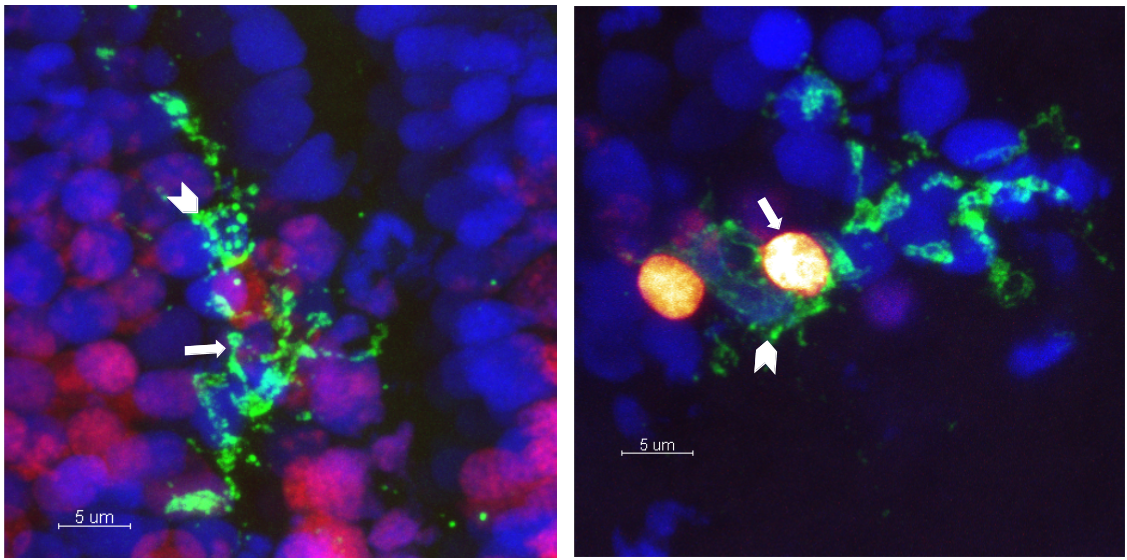
\includegraphics[width=1.\textwidth]{cmz/4C4engulfment.png}}    
    \caption{{\bf 4C4+ microglia associate with and engulf EdU-labelled CMZ contributions in the specified neural retina}}
    Representative maximum intensity projections from confocal micrographs of 14\si{\micro\metre} coronal cryosections through 30dpf zebrafish eyes labelled at 23dpf with EdU.
    
    Blue: Hoechst 33258 nuclear counterstain. Green: Microglia labelled with 4C4 antibody. Red-orange-yellow: Intensity scale of EdU staining, indicating cellular origin in the 23dpf CMZ.

    Chevrons: microglial nuclei. Arrows: EdU-positive nuclei found within 4C4-labelled extent of microglial cell body and appendages.
    
    Methods in \autoref{ssec:CMZ4C4histo}.
    \label{4C4micrograph}
\end{figure}

\begin{table}[!ht]
    \centering
    \caption{{\bf GMC-NS evidence estimates confirm Empircal Bayes analysis of early cohort stability}}
    \begin{tabular}{|l|l|l|l|l|} \hline 
        {\bf Cohort} & {\bf Time-constant logZ} & {\bf Time-varying logZ} & {\bf logZR} & {\bf $\sigma$ Significance}\\ \hline
        Embryonic central remnant & {\bf -868.79 ± 0.79} & -950.5 ± 1.5 & 81.7 ± 1.7 & 47.9\\ \hline
        1 month CMZ & {\bf -399.78 ± 0.22} & -404.05 ± 0.38 & 4.26 ± 0.43 & 9.8\\ \hline
    \end{tabular}
    \begin{flushleft} logZ: logarithm of p(D), the marginal likelihood of the data, or model evidence. logZR: evidence ratio; positive ratios in favour of the 2-phase model. Largest evidence value bolded.
    Methods in \autoref{ssec:CMZEdU}, \autoref{ssec:GMCev}.
    Code in \autoref{ssec:a27GMC_NS}.
    \end{flushleft}
    \label{turnoverGMCtable}
\end{table}

\section{Summary: Two-phase periodisation of postembryonic CMZ activity \& functional significance of CMZ activity}
Our data is best explained by a 2-phase periodization of postembryonic CMZ activity, with an initial month-long phase of relatively rapid proliferation and lower rate of exit into the specified neural retina, followed by a second phase of slower proliferation and higher exit rate. We have established posterior distributions on likely parameter ranges that convey the uncertainty we have about them; these demonstrate that our estimates of cell cycle lengths are much more certain than of exit rates.  The population of the CMZ displays an asymmetric structure which reverses over time; we have shown this is not due to time-shifting of the two proliferative phases across anatomical axes. The proportional layer composition of CMZ-driven contributions is stable over this time, and does not display variability over the dorso-ventral axis. However, by estimating the evidence for time-stable and time-varying models of lineage contribution, we identified a decline in particular retinal lineage subtypes, particularly those of the INL, but including the GCL and ONL. This a potential explanation for the teleost postembryonic change in retinal mosaic pattern. Finally, we have shown that microglia-mediated turnover of retinal neurons is occurring at a rate too low to have a measurable effect on cohort sizes during this time.

These studies demonstrate that the niche history of the CMZ is not adequately explained by a ``frozen'' population of RPC progenitors, homeostatically recapitulating the program of development found in embryonic progenitors, as has been repeatedly advanced previously \cite{Harris1998,Wan2016}. Instead, a month-long coordinated buildup in population is followed by a concerted slowing of proliferation and increase in the rate of retinal growth in the second month of life. This establishes that the postembryonic CMZ is under a separate regulatory regime from the embryonic RPCs which contribute the central, larval remnant. This period of RPC activity requires separate modelling and investigation. If, in \textit{D. rerio}, an initially productive peripheral proliferative phase is followed by a second phase decline into quiescence, this regulatory pattern may be common across vertebrate species, and its mechanistic explanations must form the basis of any attempt to entrain endogenous mammalian peripheral retinal stem cells for regenerative medicine.

We are interested in identifying macromolecular factors involved in the control of proliferation and fate specification of CMZ RPCs. These analyses suggest that these may be most profitably investigated at different ages. If we take the phase transition times estimated in \autoref{sec:sliceGMC} to be the most reliable in this chapter, this would suggest that factors implicated in proliferative control would be best identified by assays bracketing the transition time at ~35dpf; we would expect the rate of change of macromolecular correlates of cycle activity to be greatest around this time. There seems to be little spatial structure apparent in proliferative activity, and it would be unnecessary to break out these data by anatomical location, as the population size asymmetry is smallest at this time.

Overall, the data collected thus far provide the weakest support for hypotheses about RPC fate specification and niche exit. This emphasizes the sense in which proliferative and specificative activities of RPCs must be treated separately, since separate datasets, more carefully calibrated than the crude anatomical estimates used here, will be required to estimate parameters related to RPC contribution to the retina more precisely. While we were able to demonstrate an overall change in lineage subtype contribution, these pulse-chase data were not able to inform the analysis of niche exit rate. The use of saturating labelling concentrations and times in our lineage tracing experiments prevent gleaning more information about niche exit from them. The use of multiple, separately labelled thymidine analogues administered in pulses separated by a day could be a cost-effective way to inform models of niche exit and retinal contribution of the later postembryonic CMZ. Ultimately, useful explanations of retinal lineage contribution are likely to require more explicit spatial representation in order to incorporate physical effects, signalling hypotheses, and the like.

In addition to discovering unique features of postembryonic CMZ activity, we have proved out a general logic for Bayesian evaluation and selection of arbitrary biological models, which can inform both future experiments as well as modelling and theoretical choices. For instance, the slice model proves to be a more successful way to combine population and morphological information to answer questions about CMZ population structure, than are abstract whole-population models of the CMZ. Given the relative ease of producing datasets for such models, we would likely do well to establish a multiple-label thymidine analogue experimental paradigm that uses this model form for analysis. From the foregoing analyses, we conclude that treating the CMZ population as a combined unit with shared proliferative parameter evolution is likely well justified, suggesting that much of the apparent complexity of the niche's population history can be usefully abstracted away.